The main purpose of this section is to describe the dynamic behavior of Travlendar+ system when the main features are utilized. In particular we will highlight the interactions between every sub component of our system.
\subsection{Login}
			\begin{figure}[H]
				\noindent\makebox[\textwidth]{
				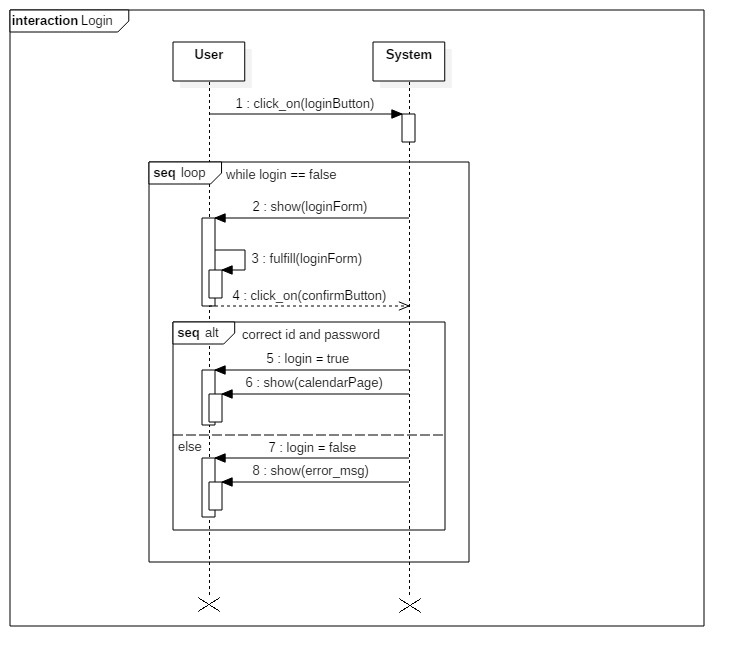
\includegraphics[scale=0.6]{sequence_diagrams/login.png}}
				\caption{Sequence Diagram - Login}
			\end{figure}
			The login operation is performed only the first time that the application is used in a new device. 
			The \textit{system} calculates a univocal code that is returned to the client and stored in the \textit{local DB}. In this way the client can identify himself during future requests. 
			The encryption function, specified in this diagram, will be specified below in the document (see section \ref{subsect:Encryption}).
\subsection{Authentication functions for each operation}
	\begin{figure}[H]
		\noindent\makebox[\textwidth]{%
		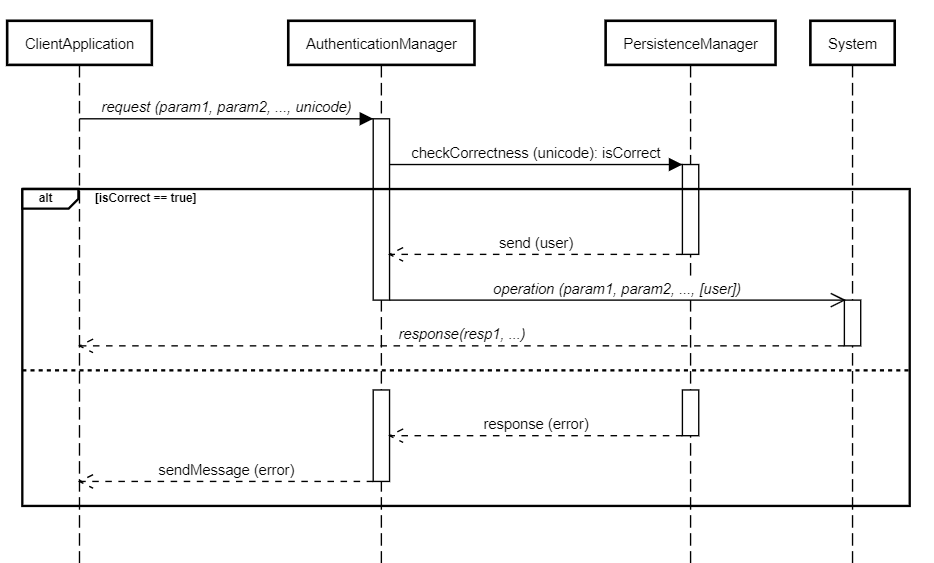
\includegraphics[width=\paperwidth,height=\paperheight,keepaspectratio]{sequence_diagrams/for_each_operation.png}}
	\caption{Sequence Diagram - Authentication}
	\end{figure}
		This is a sample of how a generic request is taken into account by the system: the \textit{Client} sends the univocal code with the other parameters of a request and the \textit{Authentication Manager} performs the check. 
		The \textit{Authentication Manager} forwards the request toward his destination only if the univocal code is correctly recognized, otherwise it reject the request.
\subsection{Create event}
	\begin{figure}[H]
		\noindent\makebox[\textwidth]{%
		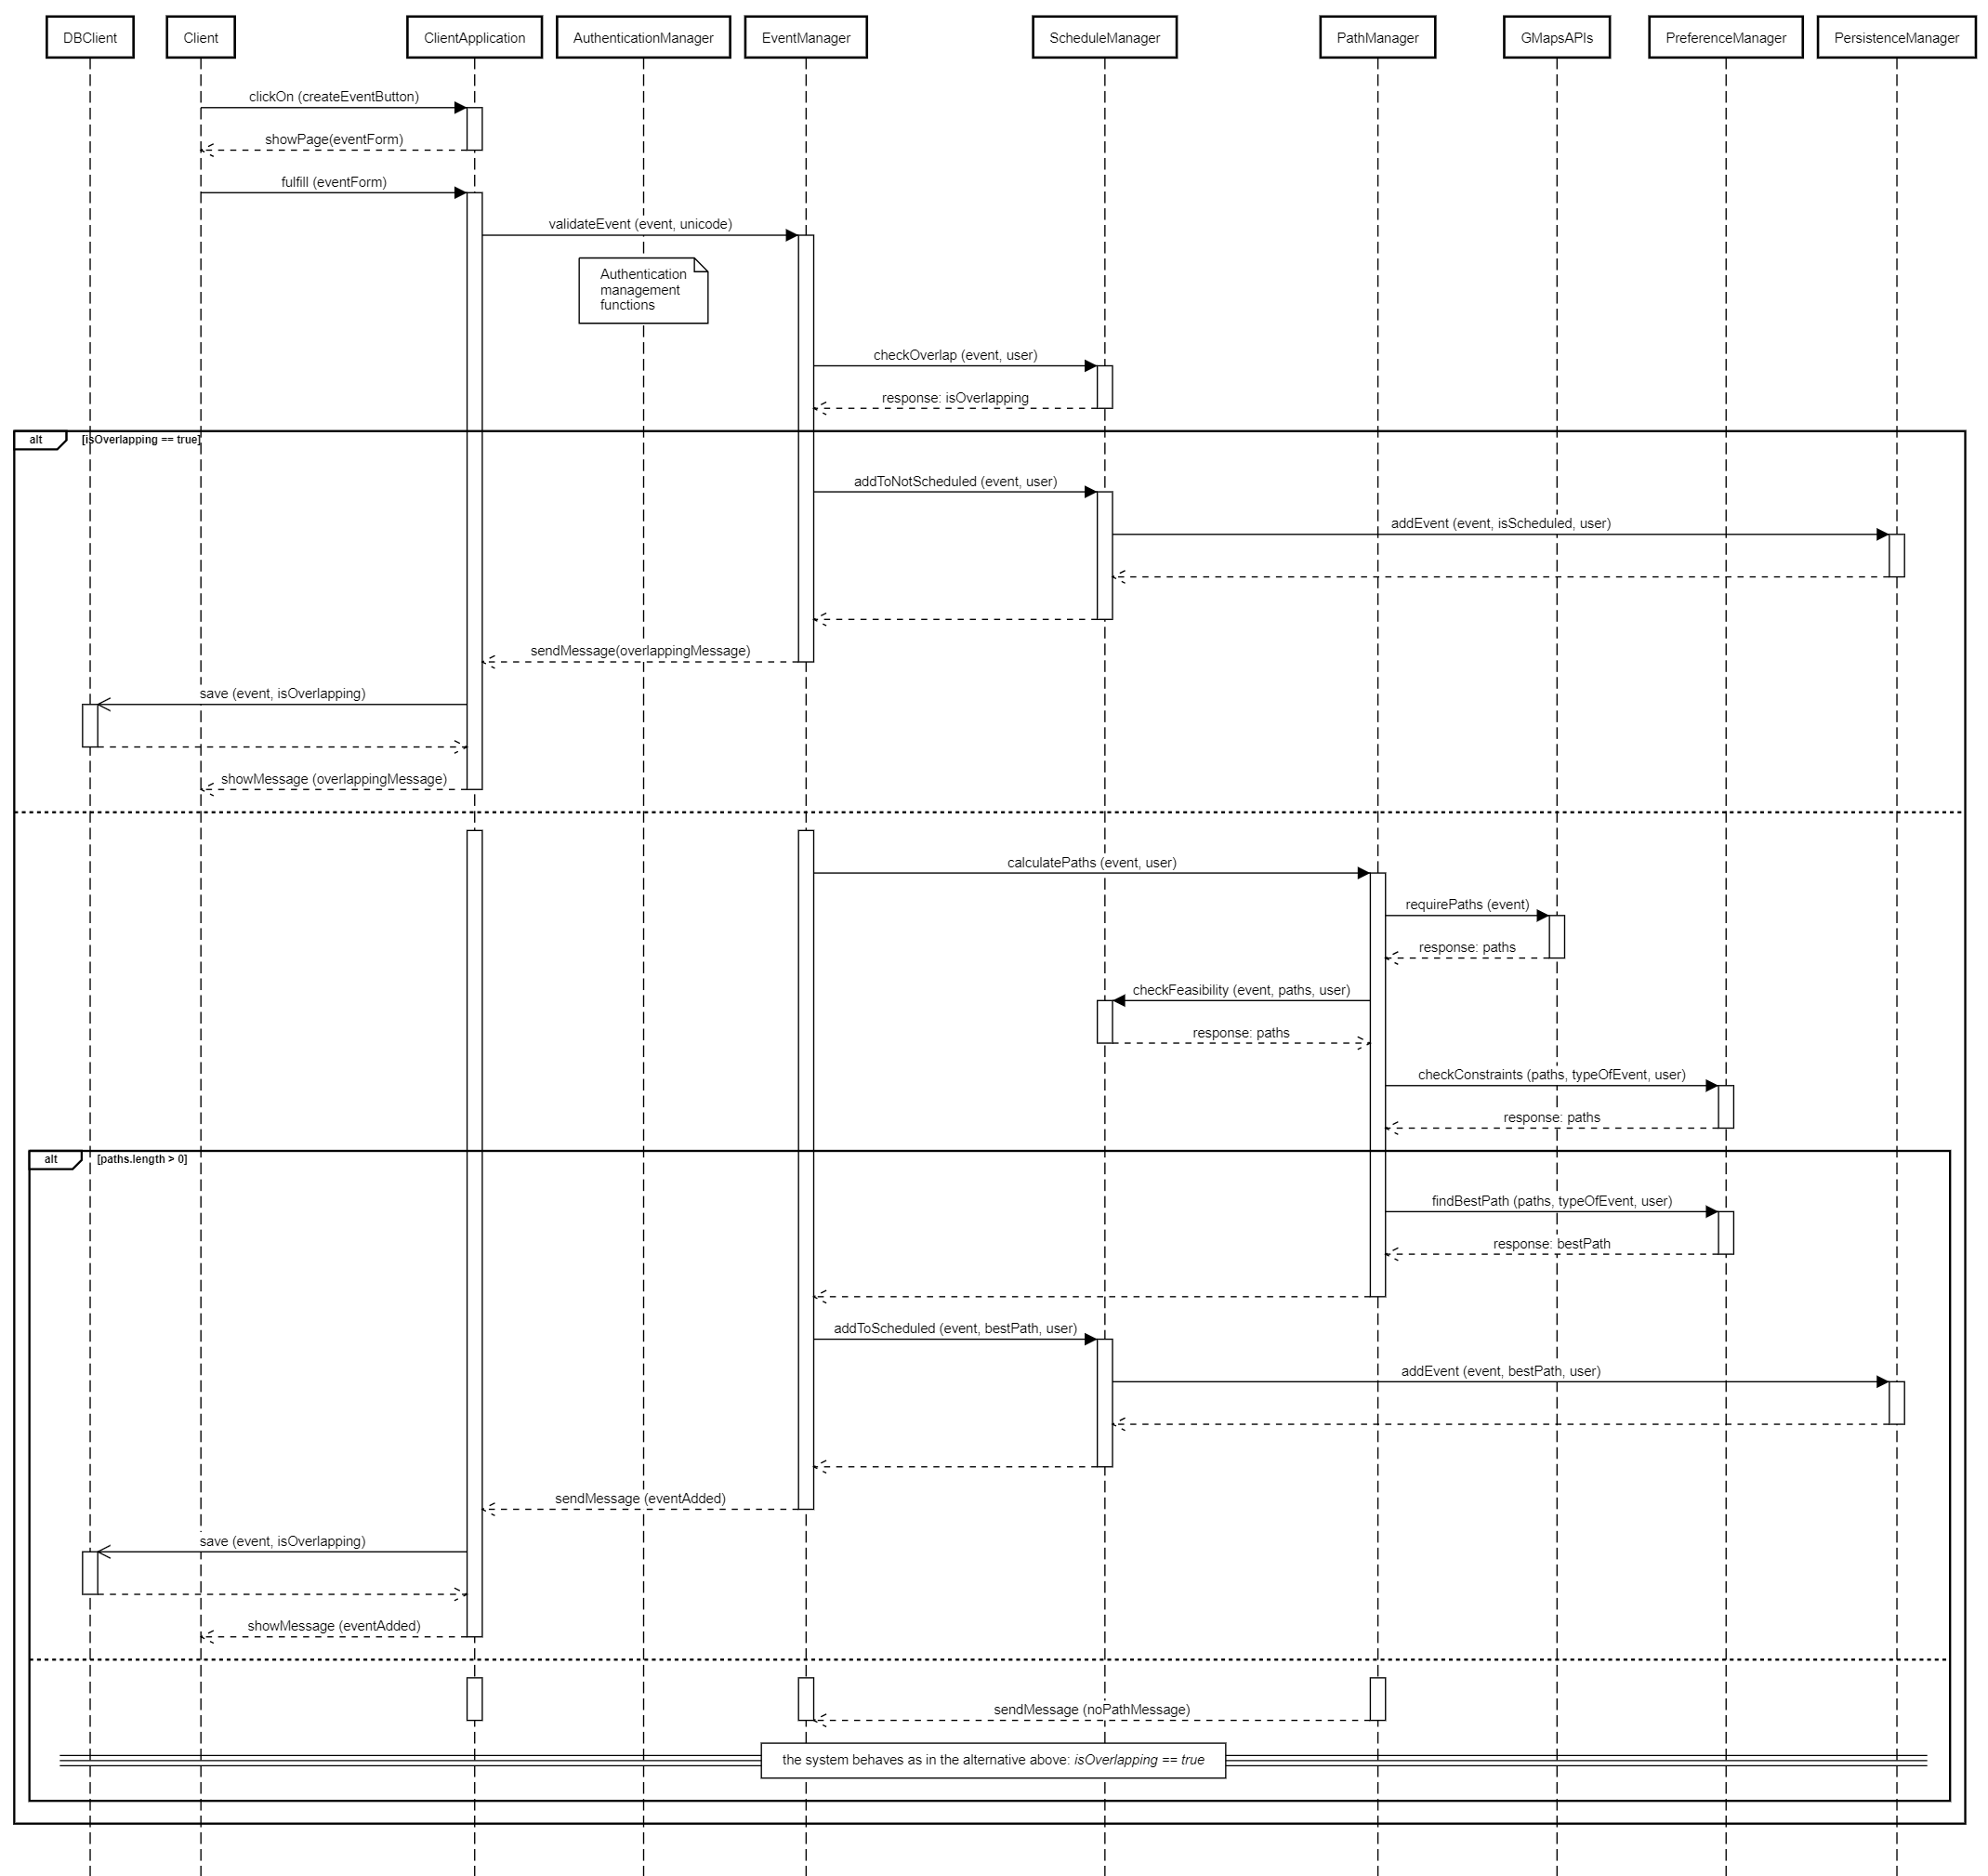
\includegraphics[width=\paperwidth,height=\paperheight,keepaspectratio]{sequence_diagrams/create_event.png}}
		\caption{Sequence Diagram - Create event}
	\end{figure}
\subsection{Arrange trip}
	\begin{figure}[H]
		\noindent\makebox[\textwidth]{%
		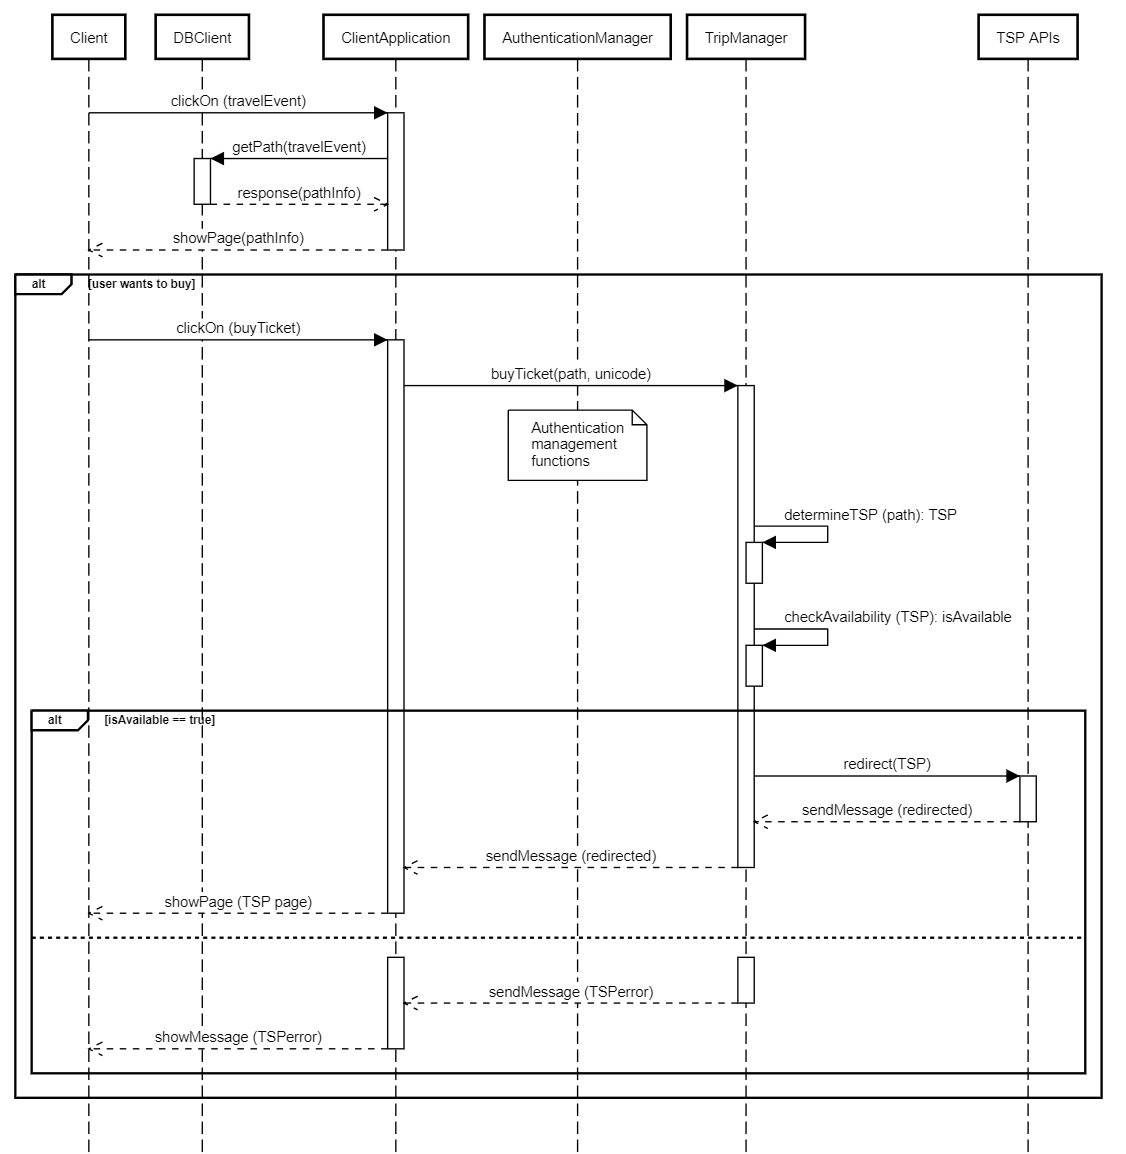
\includegraphics[width=\paperwidth,height=\paperheight,keepaspectratio]{sequence_diagrams/arrange_trip.png}}
		\caption{Sequence Diagram - Arrange trip}
	\end{figure}
\subsection{Obtain feasible paths}
	\begin{figure}[H]
		\noindent\makebox[\textwidth]{%
		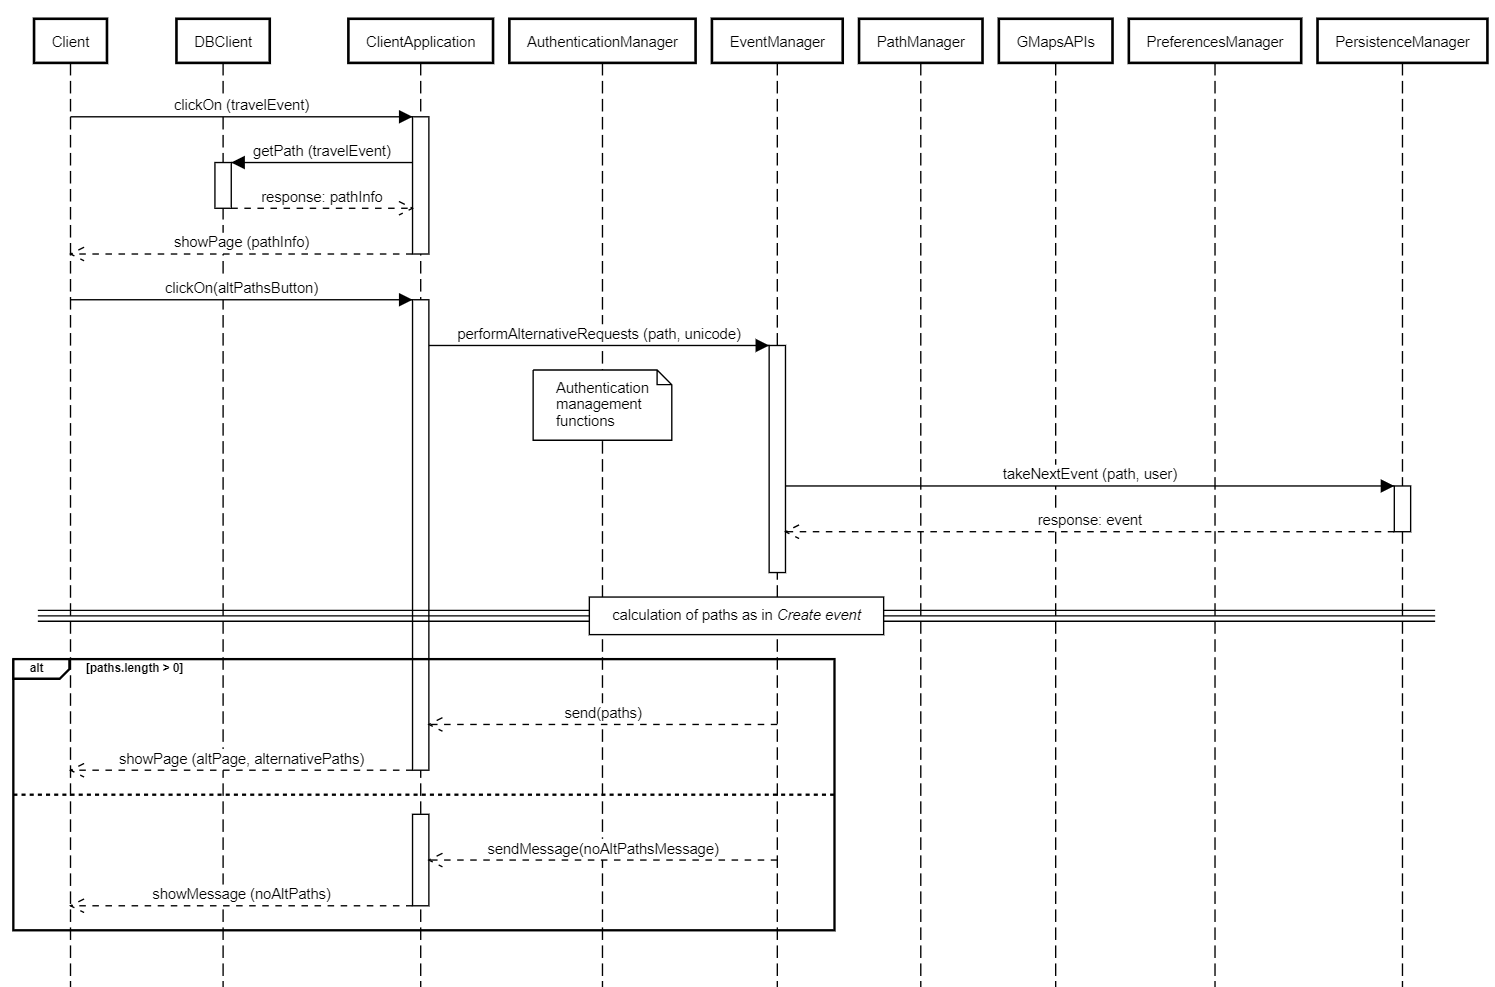
\includegraphics[width=\paperwidth,height=\paperheight,keepaspectratio]{sequence_diagrams/obtain_feasible_paths.png}}
		\caption{Sequence Diagram - Obtain feasible paths}
	\end{figure}
		Only the selected path is stored into \textit{local and server DBs}, so if a user wants to see alternative feasible paths, a new request of feasible paths is to be performed. 
		The \textit{system} obtains the event related to the path and then calculates the feasible alternatives with its internal logic and also trough the invocations of \textit{GMaps} functions. The system also checks feasibility and constraints of the obtained paths. Obviously not only the best path is returned to the \textit{client}.
\subsection{Choose between overlapping events}
	\begin{figure}[H]
		\noindent\makebox[\textwidth]{%
		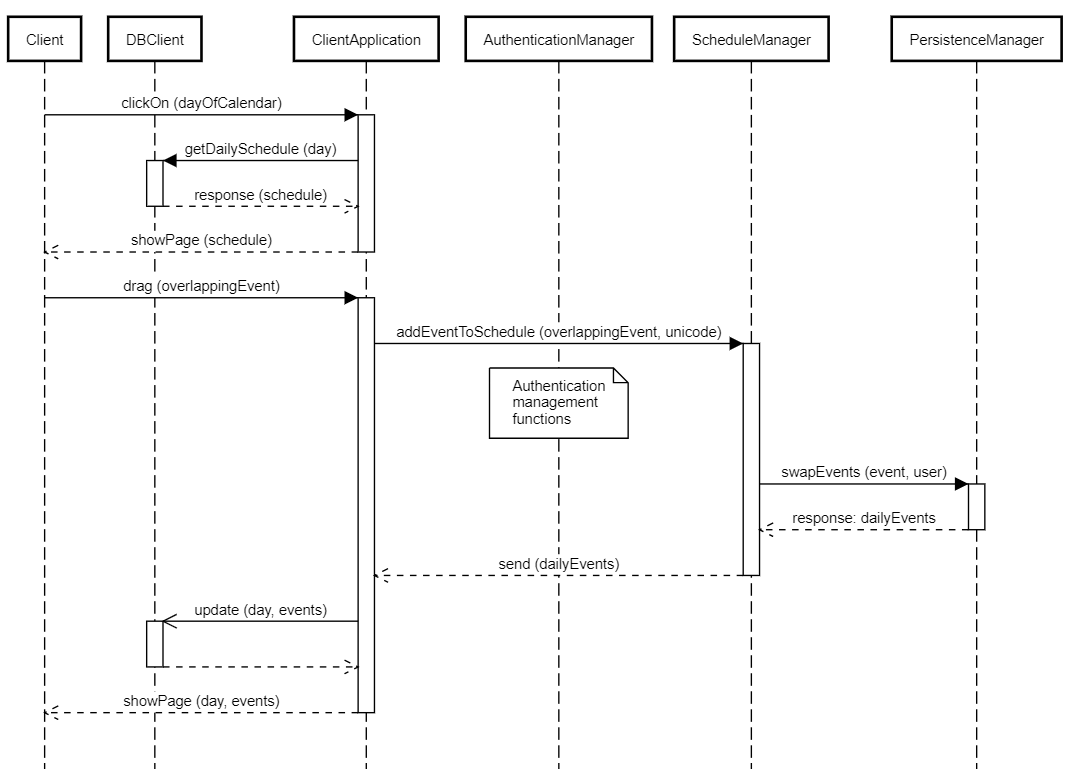
\includegraphics[width=\paperwidth,height=\paperheight,keepaspectratio]{sequence_diagrams/choose_between_overlapping_events.png}}
		\caption{Sequence Diagram - Choose between overlapping events}
	\end{figure}
\subsection{Strike announcement}
	\begin{figure}[H]
		\noindent\makebox[\textwidth]{%
		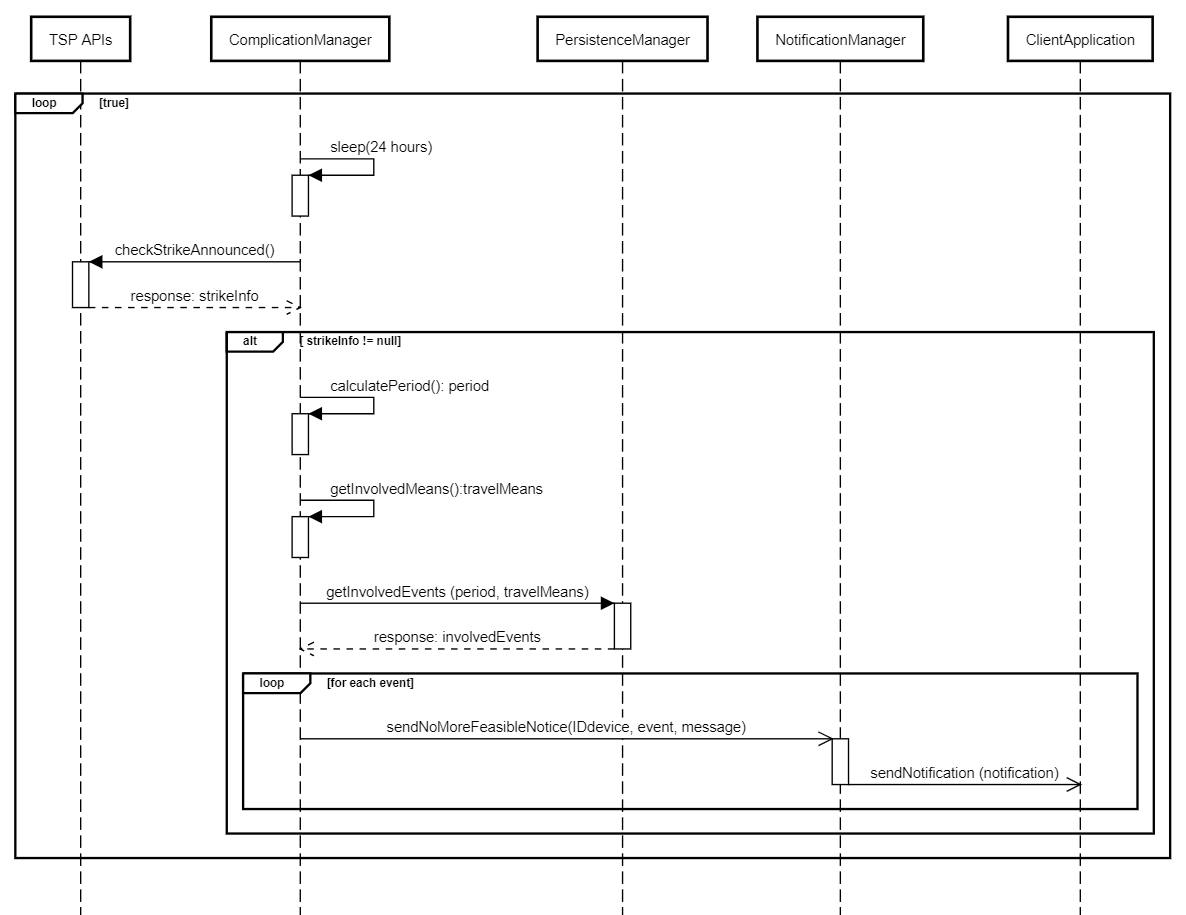
\includegraphics[width=\paperwidth,height=\paperheight,keepaspectratio]{sequence_diagrams/strike_announcement.png}}
		\caption{Sequence Diagram - Strike announcement}
	\end{figure}
		The \textit{Complication Manager} every day performs a list of operations, one of them is to check if a strike for the following days is announced. 
		In case of strike a notification is sent for each event stored in the \textit{database} that is involved: several notifications can be sent to the same user. 
		If the user opens the notification, \textit{obtain feasible paths} function, related to the involved event, is to be invoked.